%% Plantilla para la Práctica 4 en LaTeX.
%% Estructuras Discretas, 2017-1
%% Facultad de Ciencias, UNAM
%% Profa: Laura Freidberg Gojman
%% Ayudante: José Ricardo Rodríguez Abreu
%% Ayudante de lab: Albert Manuel Orozco Camacho

%% Author: AlOrozco53
%% Version: 0.0

%% Comienza el preámbulo de la presentación
\documentclass[hyperref={pdfpagelayout=SinglePage}]{beamer} %% clase de LaTeX utilizada para hacer diapositivas
\usetheme{Warsaw} %% tema visual de la presentación
%% \usecolortheme{dolphin} %% combinación de colores para el tema visual
\usepackage[utf8]{inputenc} %% codificación para la inserción acentos y otros carácteres especiales
\usepackage[T1]{fontenc} %% codificación para la impresión de acentos y otros carácteres especiales
\usepackage{graphicx} %% paquete para el manejo de imágenes y gráficos externos
\usepackage{float} %% paquete que mejora la interfaz para el manejo de objetos como tablas y figuras
\usepackage{wrapfig} %% paquete que permite que el texto se ajuste entorno a figuras y tablas
\usepackage[normalem]{ulem} %% paquete que maneja varios tipos de subrayado

%% Los siguientes paquetes sirven para utilizar símbolos especiales (principalmente de matemáticas)
\usepackage{amsmath}
\usepackage{textcomp}
\usepackage{marvosym}
\usepackage{wasysym}
\usepackage{amssymb}
\usepackage{amsthm}

\usepackage{hyperref} %% paquete para manejo de hipervínculos
\tolerance=1000 %% manejo de saltos de línea
\usepackage[english, spanish]{babel} %% paquete que administra reglas y caracterísitcas de acuerdo a los idiomas especificados

%% Colores
\PassOptionsToPackage{svgnames,smaller}{xcolor}
\usepackage[svgnames,smaller]{xcolor}

%% Varias columnas
%% \usepackage{multicol}

%% Incrementa el nivel de comandos de sección que deben ser mostrados en el índice
\setcounter{tocdepth}{4}
\setcounter{secnumdepth}{4}

\graphicspath{{../img/}} %% directorio donde se encuentran las imágenes

%% Configuración del pie de página de cada diapositiva
\setbeamertemplate{footline}{
  \leavevmode%
  \hbox{%
    \begin{beamercolorbox}[wd=.4\paperwidth,ht=2.25ex,dp=1ex,center]{author in head/foot}%
      \usebeamerfont{author in head/foot}\tiny \insertshortauthor
    \end{beamercolorbox}%
    \begin{beamercolorbox}[wd=.6\paperwidth,ht=2.25ex,dp=1ex,center]{title in head/foot}%
      \usebeamerfont{title in head/foot}\insertshorttitle\hspace*{3em}
      \insertframenumber{} / \inserttotalframenumber\hspace*{1ex}
  \end{beamercolorbox}}%
  \vskip0pt%
}

%% Título
\title[Practica 4]{Practica 4}

%% Subtítulo
%% \subtitle {Plantilla}

%% Autores
\author[Angela Janin, Luis Alberto]{
  \texttt{\href{mailto:angelajanin@ciencias.unam.mx}{Angeles Martinen Angela Janin}}\\
  \and
  \texttt{\href{mailto:luis_martinez98@ciencias.unam.mx}{Martinez Monroy Luis Alberto}}
}

%% Fecha de hoy
\date{\today}

%% Fin del preámbulo de la presentación

%% Comienza el cuerpo de la presentación
\begin{document}

%% Diapositiva para el título
\begin{frame}
  \titlepage
\end{frame}

%% Diapositiva para el índice de la presentación
\begin{frame}
  \frametitle{Índice}
  \tableofcontents
\end{frame}

\section{GHC}
\subsection{Instalacion de GHC Ubuntu y/o Debian}

\begin{frame}
  \frametitle{GHC en Ubuntu y Debian}
  \framesubtitle{Instalando GHC}
  \begin{itemize}[<+->]
  \item Ingresar a terminal de Ubuntu o la termina de Debian, segun sea su caso.
  \item ejecutar la siguiente comando en la terminal:\\\begin{center}
                                                    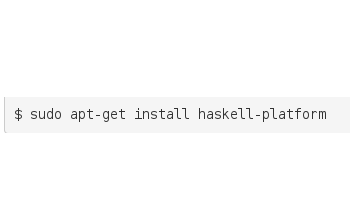
\includegraphics[width=6cm]{ghcubuntu.png}
                                                \end{center}
  \item una vez ejecutado el comando, ya estara instalada en nuestro sistema

  \end{itemize}
\end{frame}
\subsection{Instalacion de GHC Fedora}

\begin{frame}
  \frametitle{GHC en Fedora}
  \framesubtitle{Instalando GHC}
  \begin{itemize}[<+->]
  \item Ingresar a terminal de Fedora 
  \item ejecutar la siguiente comando en la terminal:\\\begin{center}
                                                    
\includegraphics[width=6cm]{ghcfedora.png}
                                                \end{center}
  \item una vez ejecutado el comando, ya estara instalada en nuestro sistema

  \end{itemize}
\end{frame}
\subsection{Utilizando ghci en tu computadora} 
\begin{frame}
  \frametitle{GHC en uso}
  \framesubtitle{Como ejecutar el modo interacivo en terminal}
  \begin{itemize}[<+->]
  \item1.- Abrimos la terminal.
  \item2.- ejecutamos el comando "ghci".
  \item3.- una vez ejecutado el comando, podemos empezar a  escribir scrips de HASKELL
  \end{itemize}
\end{frame}
\subsection{Compilacion de un archivo .hs} 
\begin{frame}
  \frametitle{ghci para compilar}
  \framesubtitle{uso del modo interactivo en un archivo .hs}
  \begin{itemize}[<+->]
  \item1.- Abrimos la terminal.
  \item2.- Nos ubicamos en la terminal en el directorio donde se encuentra nuestro archivo.hs
  \item3.- ejecutamos el comando ghci.
  \item4.- Una vez ya ejecutado el comando teclearemos ":l nombreachivo.hs"
  \item5.- Ya hecho esto, se ejecutará nuestro archivo.hs
  \item6.- si se modifica el archivo.hs, hay que volverlo a cargar a nuestro compilador repitiendo el paso 4.
  \end{itemize}
\end{frame}

\section{Funcion Factorial Haskell}
\begin{frame}
  \frametitle{Funcion factorial}
  \framesubtitle{Código Haskell}
  \begin{block}{Código Haskell para determinar un factorial}
  \begin{center}
    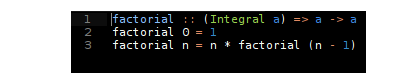
\includegraphics[width=8cm]{factorial.png}
  \end{center}
                                                
\end{block}
\end{frame}



\end{document}
%% Fin del cuerpo de la presentación
